\chapter{Specifikacija programske potpore}
		
	\section{Funkcionalni zahtjevi}
			
			\noindent \textbf{Dionici:}
			
			\begin{packed_enum}
				
				\item Vlasnik web portala (naručitelj)
				\item Klijenti web portala				
				\item Administrator
				\item Razvojni tim
				
			\end{packed_enum}
			
			\noindent \textbf{Aktori i njihovi funkcionalni zahtjevi:}
			
			
			\begin{packed_enum}
				\item  \underbar{Neregistrirani/neprijavljeni korisnik (inicijator) može:}
				
				\begin{packed_enum}
					
					\item pregledavati recepte temeljem kategorija
					\item se registrirati u sustav, stvoriti korisnički račun za koji su mu potrebni
						  korisničko ime, lozinka, ime, prezime, broj mobitela, adresa elektroničke pošte
					
				\end{packed_enum}

				\item  \underbar{Klijent (registriran i prijavljen korisnik) (inicijator) može:}
				
				\begin{packed_enum}
					
					\item pregledavati recepte temeljem kategorija
					\item objavljivati vlastite recepte
					\begin{packed_enum}
						\item komunicirati s ostalim klijentima
					\end{packed_enum}
					\item označavati tuđe recepte
					\item komentirati tuđe recepte
					\item spremati recepte za buduću referencu
					\item pratiti ostale autore
					\item pregledavati i mijenjati osobne podatke
					\item izbrisati svoj korisnički račun
					
				\end{packed_enum}

				\item  \underbar{Vlasnik (inicijator) može:}
				
				\begin{packed_enum}
					\item \textbf{*sva funkcionalnost Klijenta w/o brisanje svog računa*}
					\item brisati neželjene recepte
					\item brisati neželjene komentare
					\item brisati/dodavati kategorije
				\end{packed_enum}

				\item  \underbar{Administrator (inicijator) može:}
				
				\begin{packed_enum}
					\item \textbf{*sva funkcionalnost Vlasnika w/o funckionalost klijenta*}
					\item vidjeti popis svih registriranih korisnika i njihovih osobnih podataka
	 				\begin{packed_enum}
						\item mijenjati korisničke podatke
					\end{packed_enum}
					\item brisati korisnike i mijenjati im razinu pristupa aplikaciji (klijent, vlasnik)
				\end{packed_enum}
			
				\item  \underbar{Baza podataka (sudionik):}
				
				\begin{packed_enum}
					
					\item pohranjuje sve podatke o korisnicima i njihovim ovlastima
					\item pohranjuje sve podatke o receptima i kategorijama
					
				\end{packed_enum}
			\end{packed_enum}
			
			\eject 
			
			
				
			\subsection{Obrasci uporabe}				
				\subsubsection{Opis obrazaca uporabe}					

					\noindent \underbar{\textbf{UC1 - Pregled recepata}}
					\begin{packed_item}
	
						\item \textbf{Glavni sudionik: } Korisnik, klijent
						\item  \textbf{Cilj:} Pregledati recepte ovisno o odabranim kategorijama
						\item  \textbf{Sudionici:} Baza podataka
						\item  \textbf{Preduvjet:} -
						\item  \textbf{Opis osnovnog tijeka:}
						
						\item[] \begin{packed_enum}
	
							\item Kategorije recepata su prikazane prilikom učitavanja aplikacije
							\item Korisnik/Klijent odabire željene kategorije 
							\item Prikazuju se recepti iz željenih kategorija
						\end{packed_enum}
					\end{packed_item}

					\noindent \underbar{\textbf{UC2 - Registracija}}
					\begin{packed_item}
	
						\item \textbf{Glavni sudionik: } Korisnik
						\item  \textbf{Cilj:} Stvoriti korisnički račun za pristup sustavu
						\item  \textbf{Sudionici:} Baza podataka
						\item  \textbf{Preduvjet:} -
						\item  \textbf{Opis osnovnog tijeka:}
						
						\item[] \begin{packed_enum}
	
							\item Korisnik odabire opciju za registraciju
							\item Korisnik unosi potrebne korisničke podatke 
							\item Korisnik prima obavijest o uspješnoj registraciji
						\end{packed_enum}
						
						\item  \textbf{Opis mogućih odstupanja:}
						
						\item[] \begin{packed_item}
	
							\item[2.a] Odabir već zauzetog korisničkog imena i/ili e-maila, unos 
							korisničkog podatka u nedozvoljenom formatu ili pružanje neispravnoga e-maila
							\item[] \begin{packed_enum}
								
								\item Sustav obavještava korisnika o neuspjelom upisu i vraća ga na 
								stranicu za registraciju
								\item Korisnik mijenja potrebne podatke te završava unos ili odustaje od
								registracije
								
							\end{packed_enum}
						\end{packed_item}
					\end{packed_item}

					\noindent \underbar{\textbf{UC3 - Prijava u sustav}}
					\begin{packed_item}
	
						\item \textbf{Glavni sudionik: } Klijent
						\item  \textbf{Cilj:} Dobiti pristup korisničkom sučelju
						\item  \textbf{Sudionici:} Baza podataka
						\item  \textbf{Preduvjet:} UC2 - Registracija
						\item  \textbf{Opis osnovnog tijeka:}
						
						\item[] \begin{packed_enum}
	
							\item Unos korisničkog imena i lozinke
							\item Potvrda o ispravnosti unesenih podataka 
							\item Pristup korisničkim funkcijama
						\end{packed_enum}
						
						\item  \textbf{Opis mogućih odstupanja:}
						
						\item[] \begin{packed_item}
	
							\item[2.a] Neispravno korisničko ime/lozinka
							\item[] \begin{packed_enum}
								
								\item Sustav obavještava korisnika o neuspjelom upisu i vraća ga na
								stranicu za prijavu
								
							\end{packed_enum}
						\end{packed_item}
					\end{packed_item}

					\noindent \underbar{\textbf{UC4 - Pregled osobnih podataka}}
					\begin{packed_item}
	
						\item \textbf{Glavni sudionik: } Klijent
						\item  \textbf{Cilj:} Pregledati osobne podatke
						\item  \textbf{Sudionici:} Baza podataka
						\item  \textbf{Preduvjet:} UC3 - Prijava u sustav
						\item  \textbf{Opis osnovnog tijeka:}
						
						\item[] \begin{packed_enum}
	
							\item Klijent odabire opciju osobni podatci
							\item Aplikacija prikazuje osobne podatke klijenta
						
						\end{packed_enum}
					\end{packed_item}

					\noindent \underbar{\textbf{UC5 - Promjena osobnih podataka}}
					\begin{packed_item}
	
						\item \textbf{Glavni sudionik: } Klijent
						\item  \textbf{Cilj:} Promijenti osobne podatke
						\item  \textbf{Sudionici:} Baza podataka
						\item  \textbf{Preduvjet:} UC3 - Prijava u sustav
						\item  \textbf{Opis osnovnog tijeka:}
						
						\item[] \begin{packed_enum}
							
							\item Klijent pregledava osobne podatke
							\item Klijent odabire opciju za promjenu podataka
							\item Klijent mijenja svoje osobne podatke
							\item Klijent sprema promjene
							\item Podatci prolaze validaciju
							\item Baza podataka se ažurira
							
						\end{packed_enum}
						
						\item  \textbf{Opis mogućih odstupanja:}
						
						\item[] \begin{packed_item}
	
							\item[2.a] Unos neispravnih podataka
							\item[] \begin{packed_enum}
								
								\item Sustav obavještava korisnika o neuspjelom upisu i vraća ga
								na opciju za promjenu podataka
								
							\end{packed_enum}
						\end{packed_item}
					\end{packed_item}

					\noindent \underbar{\textbf{UC6 - Brisanje korisničkog računa}}
					\begin{packed_item}
	
						\item \textbf{Glavni sudionik: } Klijent
						\item  \textbf{Cilj:} Izbrisati korisnički račun
						\item  \textbf{Sudionici:} Baza podataka
						\item  \textbf{Preduvjet:} UC3 - Prijava u sustav
						\item  \textbf{Opis osnovnog tijeka:}
						
						\item[] \begin{packed_enum}
	
							\item Klijent pregledava osobne podatke
							\item Klijent odabire opciju brisanja korisničkog računa
							\item Klijent briše račun
							\item Posljedično se brišu i svi recepti te komentari klijenta
							\item Baza podataka se ažurira
							\item Otvara se stranica za registraciju
						
						\end{packed_enum}
					\end{packed_item}

					\noindent \underbar{\textbf{UC7 - Objavljivanje recepta}}
					\begin{packed_item}
	
						\item \textbf{Glavni sudionik: } Klijent
						\item  \textbf{Cilj:} Objaviti recept na web portalu
						\item  \textbf{Sudionici:} Baza podataka
						\item  \textbf{Preduvjet:} UC3 - Prijava u sustav
						\item  \textbf{Opis osnovnog tijeka:}
						
						\item[] \begin{packed_enum}
	
							\item Klijent odabire opciju objavi recept
							\item Klijent unosi potrebne podatke o receptu
							\item Klijent objavljuje recept
							\item Klijent prima obavijest o uspješnoj objavi recepta
							\item Šalje se obavijest svim pratiteljima klijenta/autora
							\item Baza podataka se ažurira
							\item Otvara se stranica sa receptima korisnika
						\end{packed_enum}

						\item  \textbf{Opis mogućih odstupanja:}
						
						\item[] \begin{packed_item}
	
							\item[2.a] Unos neispravnih podataka
							\item[] \begin{packed_enum}
								
								\item Sustav obavještava korisnika o neuspjelom upisu i vraća ga
								na opciju za objavu recepta
								
							\end{packed_enum}
						\end{packed_item}
					\end{packed_item}

					\noindent \underbar{\textbf{UC8 - Uređivanje recepta}}
					\begin{packed_item}
	
						\item \textbf{Glavni sudionik: } Klijent
						\item  \textbf{Cilj:} Urediti recept na web portalu
						\item  \textbf{Sudionici:} Baza podataka
						\item  \textbf{Preduvjet:} UC3 - Prijava u sustav, UC7 - Objavljivanje recepta
						\item  \textbf{Opis osnovnog tijeka:}
						
						\item[] \begin{packed_enum}
							
							\item Klijent otvara stranicu sa svojim receptima
							\item Klijent odabire opciju uređivanja recepta
							\item Klijent mijenja određene podatke o receptu
							\item Klijent sprema promijene
							\item Klijent prima obavijest o uspješnoj promijeni recepta
							\item Baza podataka se ažurira
							\item Otvara se stranica sa receptima korisnika
						\end{packed_enum}

						\item  \textbf{Opis mogućih odstupanja:}
						
						\item[] \begin{packed_item}
	
							\item[3.a] Unos neispravnih podataka
							\item[] \begin{packed_enum}
								
								\item Sustav obavještava korisnika o neuspjelom upisu i vraća ga
								na opciju za objavu recepta
								
							\end{packed_enum}
						\end{packed_item}
					\end{packed_item}

					\noindent \underbar{\textbf{UC9 - Brisanje recepta}}
					\begin{packed_item}
	
						\item \textbf{Glavni sudionik: } Klijent
						\item  \textbf{Cilj:} Izbrisati recept sa web portala
						\item  \textbf{Sudionici:} Baza podataka
						\item  \textbf{Preduvjet:} UC3 - Prijava u sustav, UC7 - Objavljivanje recepta
						\item  \textbf{Opis osnovnog tijeka:}
						
						\item[] \begin{packed_enum}
							
							\item Klijent otvara stranicu sa svojim receptima
							\item Klijent odabire opciju brisanja recepta
							\item Klijent prima obavijest o uspješnom brisanju recepta
							\item Baza podataka se ažurira
							\item Klijenti koji su recept imali spremljen, više ga nemaju
							\item Otvara su stranica sa receptima korisnika
						\end{packed_enum}
					\end{packed_item}

					\noindent \underbar{\textbf{UC10 - Slanje poruke}}
					\begin{packed_item}
	
						\item \textbf{Glavni sudionik: } Klijent
						\item  \textbf{Cilj:} Poslati poruku drugom klijentu (autoru recepta) 
						\item  \textbf{Sudionici:} Baza podataka
						\item  \textbf{Preduvjet:} UC3 - Prijava u sustav
						\item  \textbf{Opis osnovnog tijeka:}
						
						\item[] \begin{packed_enum}
							
							\item Klijent odabire opciju slanja poruke drugom klijentu (autoru recepta)
							\item Klijent piše odgovarajuću poruku
							\item Klijent šalje poruku
							\item Klijent prima obavijest o uspješnom slanju poruke
							\item Baza podataka se ažurira
						\end{packed_enum}
					\end{packed_item}

					\noindent \underbar{\textbf{UC11 - Primanje poruke}}
					\begin{packed_item}
	
						\item \textbf{Glavni sudionik: } Klijent
						\item  \textbf{Cilj:} Primiti poruku od drugog klijenta 
						\item  \textbf{Sudionici:} Baza podataka
						\item  \textbf{Preduvjet:} UC3 - Prijava u sustav
						\item  \textbf{Opis osnovnog tijeka:}
						
						\item[] \begin{packed_enum}
							
							\item Klijent se prijavljuje u sustav
							\item Klijent odabire opciju provjere obavijesti
							\item Klijent čita poruku
						\end{packed_enum}
					\end{packed_item}

					\noindent \underbar{\textbf{UC12 - Komentiranje recepta}}
					\begin{packed_item}
	
						\item \textbf{Glavni sudionik: } Klijent
						\item  \textbf{Cilj:} Objaviti komentar na receptu 
						\item  \textbf{Sudionici:} Baza podataka
						\item  \textbf{Preduvjet:} UC3 - Prijava u sustav
						\item  \textbf{Opis osnovnog tijeka:}
						
						\item[] \begin{packed_enum}
							
							\item Klijent odabire recept koji želi komentirati
							\item Klijent piše željeni komentar
							\item Klijent objavljuje komentar
							\item Baza podataka se ažurira
						\end{packed_enum}

						\item  \textbf{Opis mogućih odstupanja:}
						
						\item[] \begin{packed_item}
	
							\item[3.a] Unos neispravnih podataka (dopušteni znakovi)
							\item[] \begin{packed_enum}
								
								\item Sustav obavještava korisnika o neuspjeloj objavi komentara
								
							\end{packed_enum}
						\end{packed_item}
					\end{packed_item}

					\noindent \underbar{\textbf{UC13 - Spremanje recepta}}
					\begin{packed_item}
	
						\item \textbf{Glavni sudionik: } Klijent
						\item  \textbf{Cilj:} Spremiti recept za kasniju referencu 
						\item  \textbf{Sudionici:} Baza podataka
						\item  \textbf{Preduvjet:} UC3 - Prijava u sustav
						\item  \textbf{Opis osnovnog tijeka:}
						
						\item[] \begin{packed_enum}
							
							\item Klijent odabire recept koji želi spremiti
							\item Klijent sprema recept
							\item Baza podataka se ažurira
						\end{packed_enum}
					\end{packed_item}

					\noindent \underbar{\textbf{UC14 - Micanje recepta}}
					\begin{packed_item}
	
						\item \textbf{Glavni sudionik: } Klijent
						\item  \textbf{Cilj:} Maknuti recept iz spremljenih recepata 
						\item  \textbf{Sudionici:} Baza podataka
						\item  \textbf{Preduvjet:} UC3 - Prijava u sustav, UC13 - Spremanje recepta
						\item  \textbf{Opis osnovnog tijeka:}
						
						\item[] \begin{packed_enum}
							
							\item Klijent odabire recept koji želi maknuti iz spremljenih
							\item Klijent miče recept
							\item Baza podataka se ažurira
						\end{packed_enum}
					\end{packed_item}

					\noindent \underbar{\textbf{UC15 - Označavanje recepta}}
					\begin{packed_item}
	
						\item \textbf{Glavni sudionik: } Klijent
						\item  \textbf{Cilj:} Označiti recept za kasniju referencu 
						\item  \textbf{Sudionici:} Baza podataka
						\item  \textbf{Preduvjet:} UC3 - Prijava u sustav
						\item  \textbf{Opis osnovnog tijeka:}
						
						\item[] \begin{packed_enum}
							
							\item Klijent odabire recept koji želi označiti kao jedan od svojih omiljenih
							\item Klijent označava recept
							\item Baza podataka se ažurira
						\end{packed_enum}
					\end{packed_item}

					\noindent \underbar{\textbf{UC16 - Odznačavanje recepta}}
					\begin{packed_item}
	
						\item \textbf{Glavni sudionik: } Klijent
						\item  \textbf{Cilj:} Maknuti oznaku sa recepta
						\item  \textbf{Sudionici:} Baza podataka
						\item  \textbf{Preduvjet:} UC3 - Prijava u sustav, UC14 - Označavanje recepta
						\item  \textbf{Opis osnovnog tijeka:}
						
						\item[] \begin{packed_enum}
							
							\item Klijent odabire recept kojem želi maknuti oznaku
							\item Klijent miče recept
							\item Baza podataka se ažurira
						\end{packed_enum}
					\end{packed_item}

					
					\noindent \underbar{\textbf{UC17 - Praćenje autora}}
					\begin{packed_item}
	
						\item \textbf{Glavni sudionik: } Klijent
						\item  \textbf{Cilj:} Označiti autora od kojeg želi primati obavijesti 
						\item  \textbf{Sudionici:} Baza podataka
						\item  \textbf{Preduvjet:} UC3 - Prijava u sustav
						\item  \textbf{Opis osnovnog tijeka:}
						
						\item[] \begin{packed_enum}
							
							\item Klijent odabire autora kojeg želi zapratiti, tj. od njega primati obavijesti
							\item Klijent zaprati autora
							\item Baza podataka se ažurira
						\end{packed_enum}
					\end{packed_item}

					\noindent \underbar{\textbf{UC18 - Prestanak praćenja autora}}
					\begin{packed_item}
	
						\item \textbf{Glavni sudionik: } Klijent
						\item  \textbf{Cilj:} Prestati pratiti autora, tj. od njega primati obavijesti
						\item  \textbf{Sudionici:} Baza podataka
						\item  \textbf{Preduvjet:} UC3 - Prijava u sustav, UC17 - Praćenje autora
						\item  \textbf{Opis osnovnog tijeka:}
						
						\item[] \begin{packed_enum}
							
							\item Klijent odabire autora kojeg želi prestati pratiti.
							\item Klijent prestaje pratiti autora
							\item Baza podataka se ažurira
						\end{packed_enum}
					\end{packed_item}

					\noindent \underbar{\textbf{UC19 - Slanje obavijesti}}
					\begin{packed_item}
	
						\item \textbf{Glavni sudionik: } Klijent
						\item  \textbf{Cilj:} Poslati obavijest svojim pratiteljima
						\item  \textbf{Sudionici:} Baza podataka
						\item  \textbf{Preduvjet:} UC3 - Prijava u sustav, UC7 - Objavljivanje recepta
						\item  \textbf{Opis osnovnog tijeka:}
						
						\item[] \begin{packed_enum}
							
							\item Klijent objavljuje novi recept
							\item Njegovim pratiteljima stiže obavijest
							\item Baza podataka se ažurira
						\end{packed_enum}
					\end{packed_item}

					\noindent \underbar{\textbf{UC20 - Primanje obavijesti}}
					\begin{packed_item}
	
						\item \textbf{Glavni sudionik: } Klijent
						\item  \textbf{Cilj:} Primiti obavijest praćenog autora
						\item  \textbf{Sudionici:} Baza podataka
						\item  \textbf{Preduvjet:} UC3 - Prijava u sustav, UC15 - Praćenje autora
						\item  \textbf{Opis osnovnog tijeka:}
						
						\item[] \begin{packed_enum}
							
							\item Klijent se prijavljuje u sustav
							\item Klijent odabire opciju provjere obavijesti
							\item Klijent čita obavijest
						\end{packed_enum}
					\end{packed_item}

					\noindent \underbar{\textbf{UC21 - Dodavanje kategorije}}
					\begin{packed_item}
	
						\item \textbf{Glavni sudionik: } Vlasnik, Administrator
						\item  \textbf{Cilj:} Dodati novu kategoriju recepata
						\item  \textbf{Sudionici:} Baza podataka
						\item  \textbf{Preduvjet:} UC3 - Prijava u sustav (kao jedan od sudionika)
						\item  \textbf{Opis osnovnog tijeka:}
						
						\item[] \begin{packed_enum}
							
							\item Vlasnik/Administrator se prijavljuje u sustav
							\item Vlasnik/Administrator odabire opciju dodavanja kategorija
							\item Vlasnik/Administrator dodaje novu kategoriju
							\item Baza podataka se ažurira
						\end{packed_enum}

						\item[] \begin{packed_item}
	
							\item[3.a] Unos postojeće kategorije
							\item[] \begin{packed_enum}
								
								\item Sustav obavještava korisnika o neuspjelom dodavanju 
								kategorije, vraća ga na stranicu s kategorijama
								
							\end{packed_enum}

							\item[3.b] Unos neispravnih podataka (dopušteni znakovi)
							\item[] \begin{packed_enum}
								
								\item Sustav obavještava korisnika o neuspjelom dodavanju 
								kategorije, vraća ga na stranicu s kategorijama							\end{packed_enum}
						\end{packed_item}
					\end{packed_item}

					\noindent \underbar{\textbf{UC22 - Brisanje kategorije}}
					\begin{packed_item}
	
						\item \textbf{Glavni sudionik: } Vlasnik, Administrator
						\item  \textbf{Cilj:} Izbrisati kategoriju recepata
						\item  \textbf{Sudionici:} Baza podataka
						\item  \textbf{Preduvjet:} UC3 - Prijava u sustav (kao jedan od sudionika)
						\item  \textbf{Opis osnovnog tijeka:}
						
						\item[] \begin{packed_enum}
							
							\item Vlasnik/Administrator se prijavljuje u sustav
							\item Vlasnik/Administrator odabire opciju brisanja kategorija
							\item Vlasnik/Administrator briše kategoriju
							\item Baza podataka se ažurira
						\end{packed_enum}
					\end{packed_item}

					\noindent \underbar{\textbf{UC23 - Brisanje komentara}}
					\begin{packed_item}
	
						\item \textbf{Glavni sudionik: } Vlasnik, Administrator
						\item  \textbf{Cilj:} Izbrisati komentar na recept
						\item  \textbf{Sudionici:} Baza podataka
						\item  \textbf{Preduvjet:} UC3 - Prijava u sustav (kao jedan od sudionika)
						\item  \textbf{Opis osnovnog tijeka:}
						
						\item[] \begin{packed_enum}
							
							\item Vlasnik/Administrator se prijavljuje u sustav
							\item Vlasnik/Administrator odabire komentar koji želi obrisati
							\item Vlasnik/Administrator briše komentar
							\item Baza podataka se ažurira
						\end{packed_enum}
					\end{packed_item}

					\noindent \underbar{\textbf{UC24 - Pregled korisnika}}
					\begin{packed_item}
	
						\item \textbf{Glavni sudionik: } Administrator
						\item  \textbf{Cilj:} Pregledati popis klijenata
						\item  \textbf{Sudionici:} Baza podataka
						\item  \textbf{Preduvjet:} UC3 - Prijava u sustav (kao jedan od sudionika)
						\item  \textbf{Opis osnovnog tijeka:}
						
						\item[] \begin{packed_enum}
							
							\item Administrator se prijavljuje u sustav
							\item Administrator odabire opciju pregleda korisnika
							\item Prikaže se lista svih registriranih korisnika
						\end{packed_enum}
					\end{packed_item}

					\noindent \underbar{\textbf{UC25 - Brisanje korisnika}}
					\begin{packed_item}
	
						\item \textbf{Glavni sudionik: } Administrator
						\item  \textbf{Cilj:} Obrisati korisnički račun klijenta
						\item  \textbf{Sudionici:} Baza podataka
						\item  \textbf{Preduvjet:} UC3 - Prijava u sustav (kao jedan od sudionika)
						\item  \textbf{Opis osnovnog tijeka:}
						
						\item[] \begin{packed_enum}
							
							\item Administrator se prijavljuje u sustav
							\item Administrator odabire željenog korisnika
							\item Administrator odabire opciju brisanja korisnika
							\item Korisnički račun klijenta se obriše
							\item Posljedično se brišu i svi recepti te komentari klijenta
							\item Baza podataka se ažurira
						\end{packed_enum}
					\end{packed_item}

					\noindent \underbar{\textbf{UC26 - Promjena prava korisnika}}
					\begin{packed_item}
	
						\item \textbf{Glavni sudionik: } Administrator
						\item  \textbf{Cilj:} Promijeniti razinu pristupa korisnika
						\item  \textbf{Sudionici:} Baza podataka
						\item  \textbf{Preduvjet:} UC3 - Prijava u sustav (kao jedan od sudionika)
						\item  \textbf{Opis osnovnog tijeka:}
						
						\item[] \begin{packed_enum}
							
							\item Administrator se prijavljuje u sustav
							\item Administrator odabire željenog korisnika
							\item Administrator odabire opciju promijene prava korisnika
							\item Administrator mijenja razinu pristupa korisnika
							\item Baza podataka se ažurira
						\end{packed_enum}
					\end{packed_item}
				
					
			\subsubsection{Dijagrami obrazaca uporabe}
				\begin{figure}[H]
					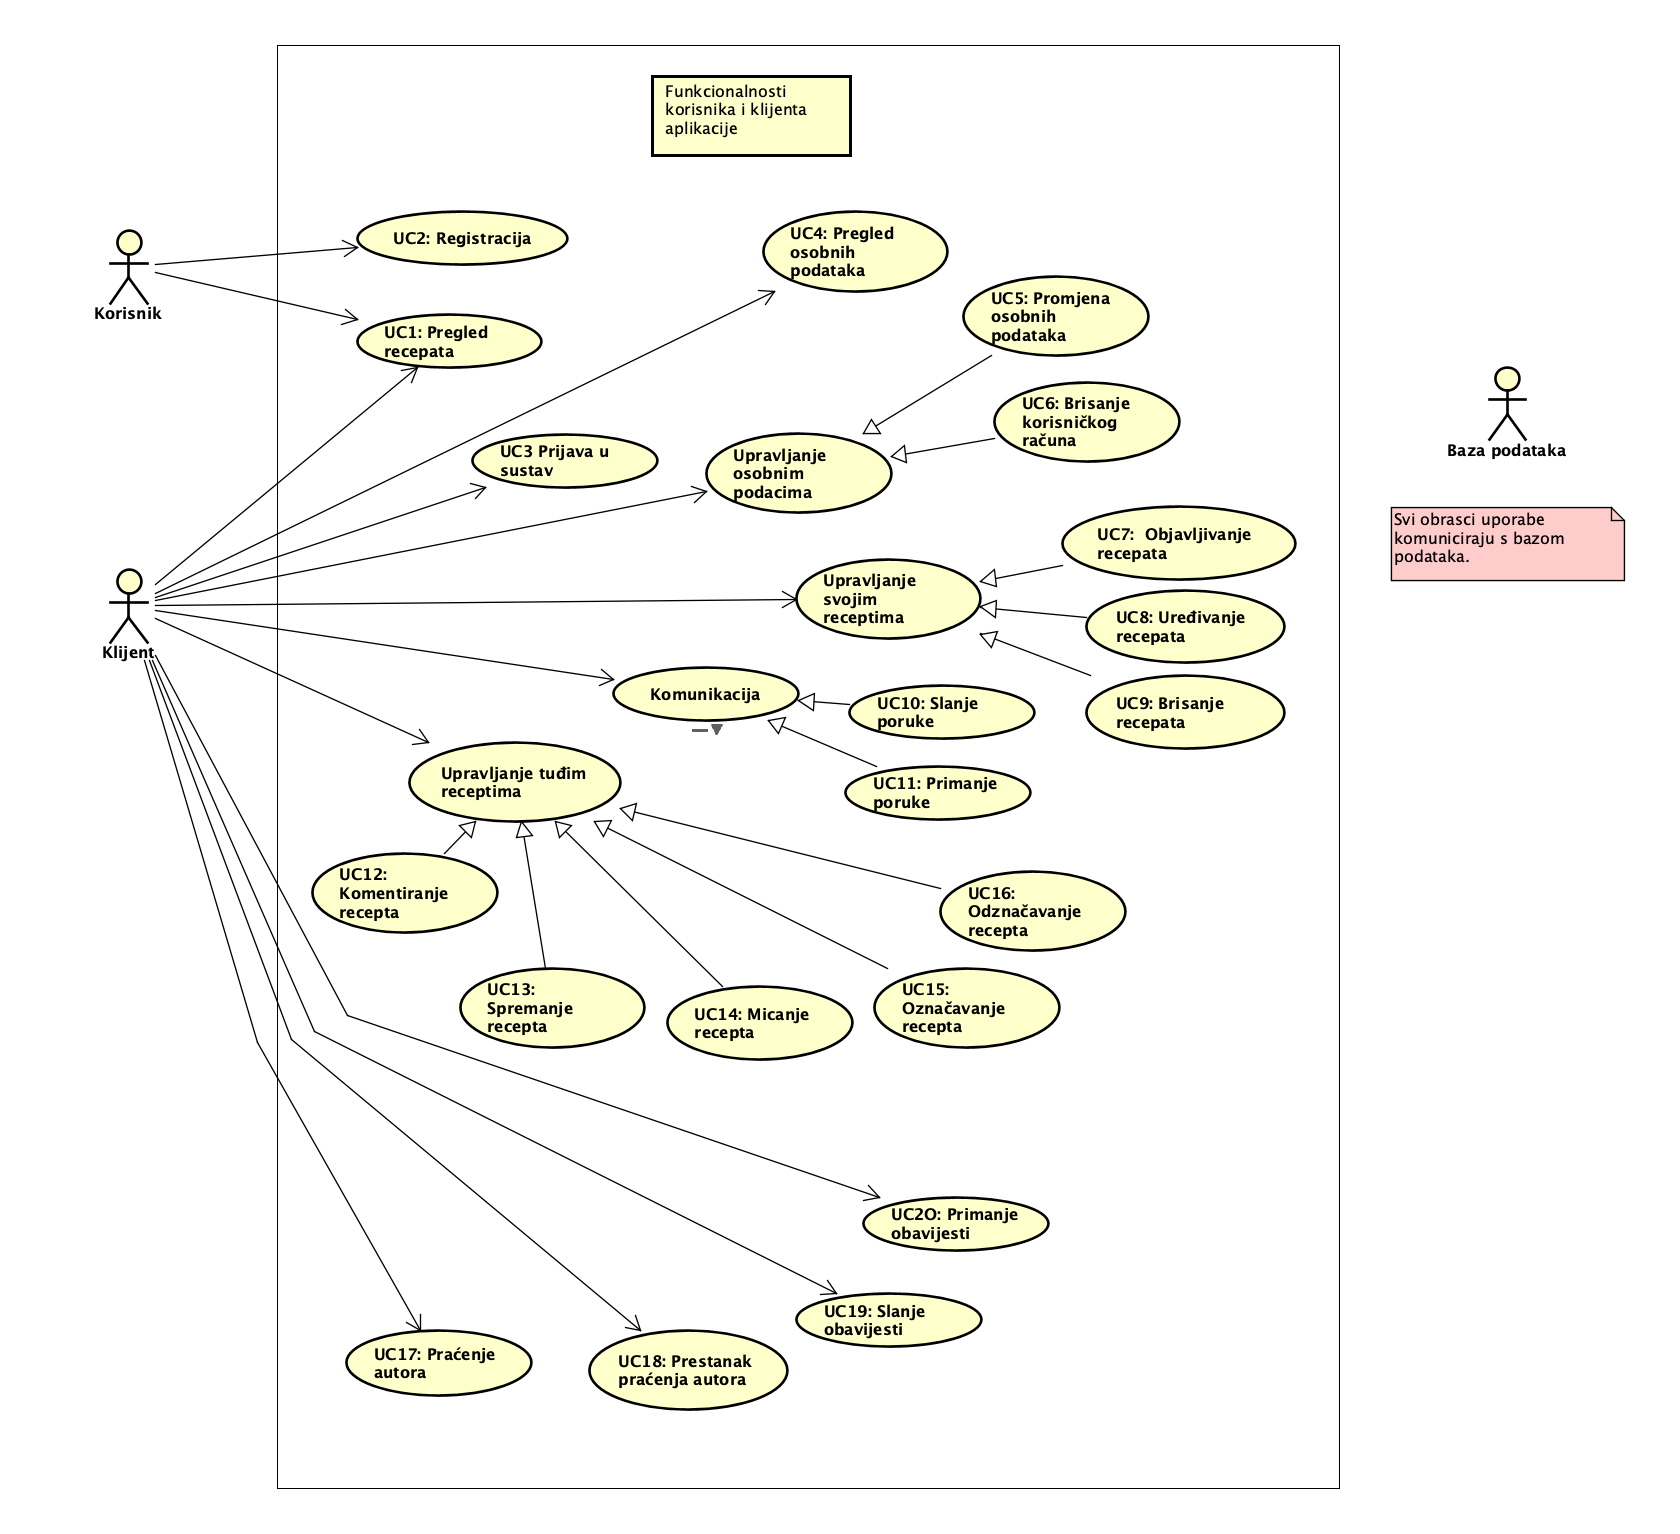
\includegraphics[scale=0.6]{dijagrami/Korisnik_klijent.png} 
					\centering
					\caption{Dijagram obrasca uporabe, funkcionalnost korisnika i klijenta}
					\label{fig:korisnik-klijent}
				\end{figure}
				\eject

				\begin{figure}[H]
					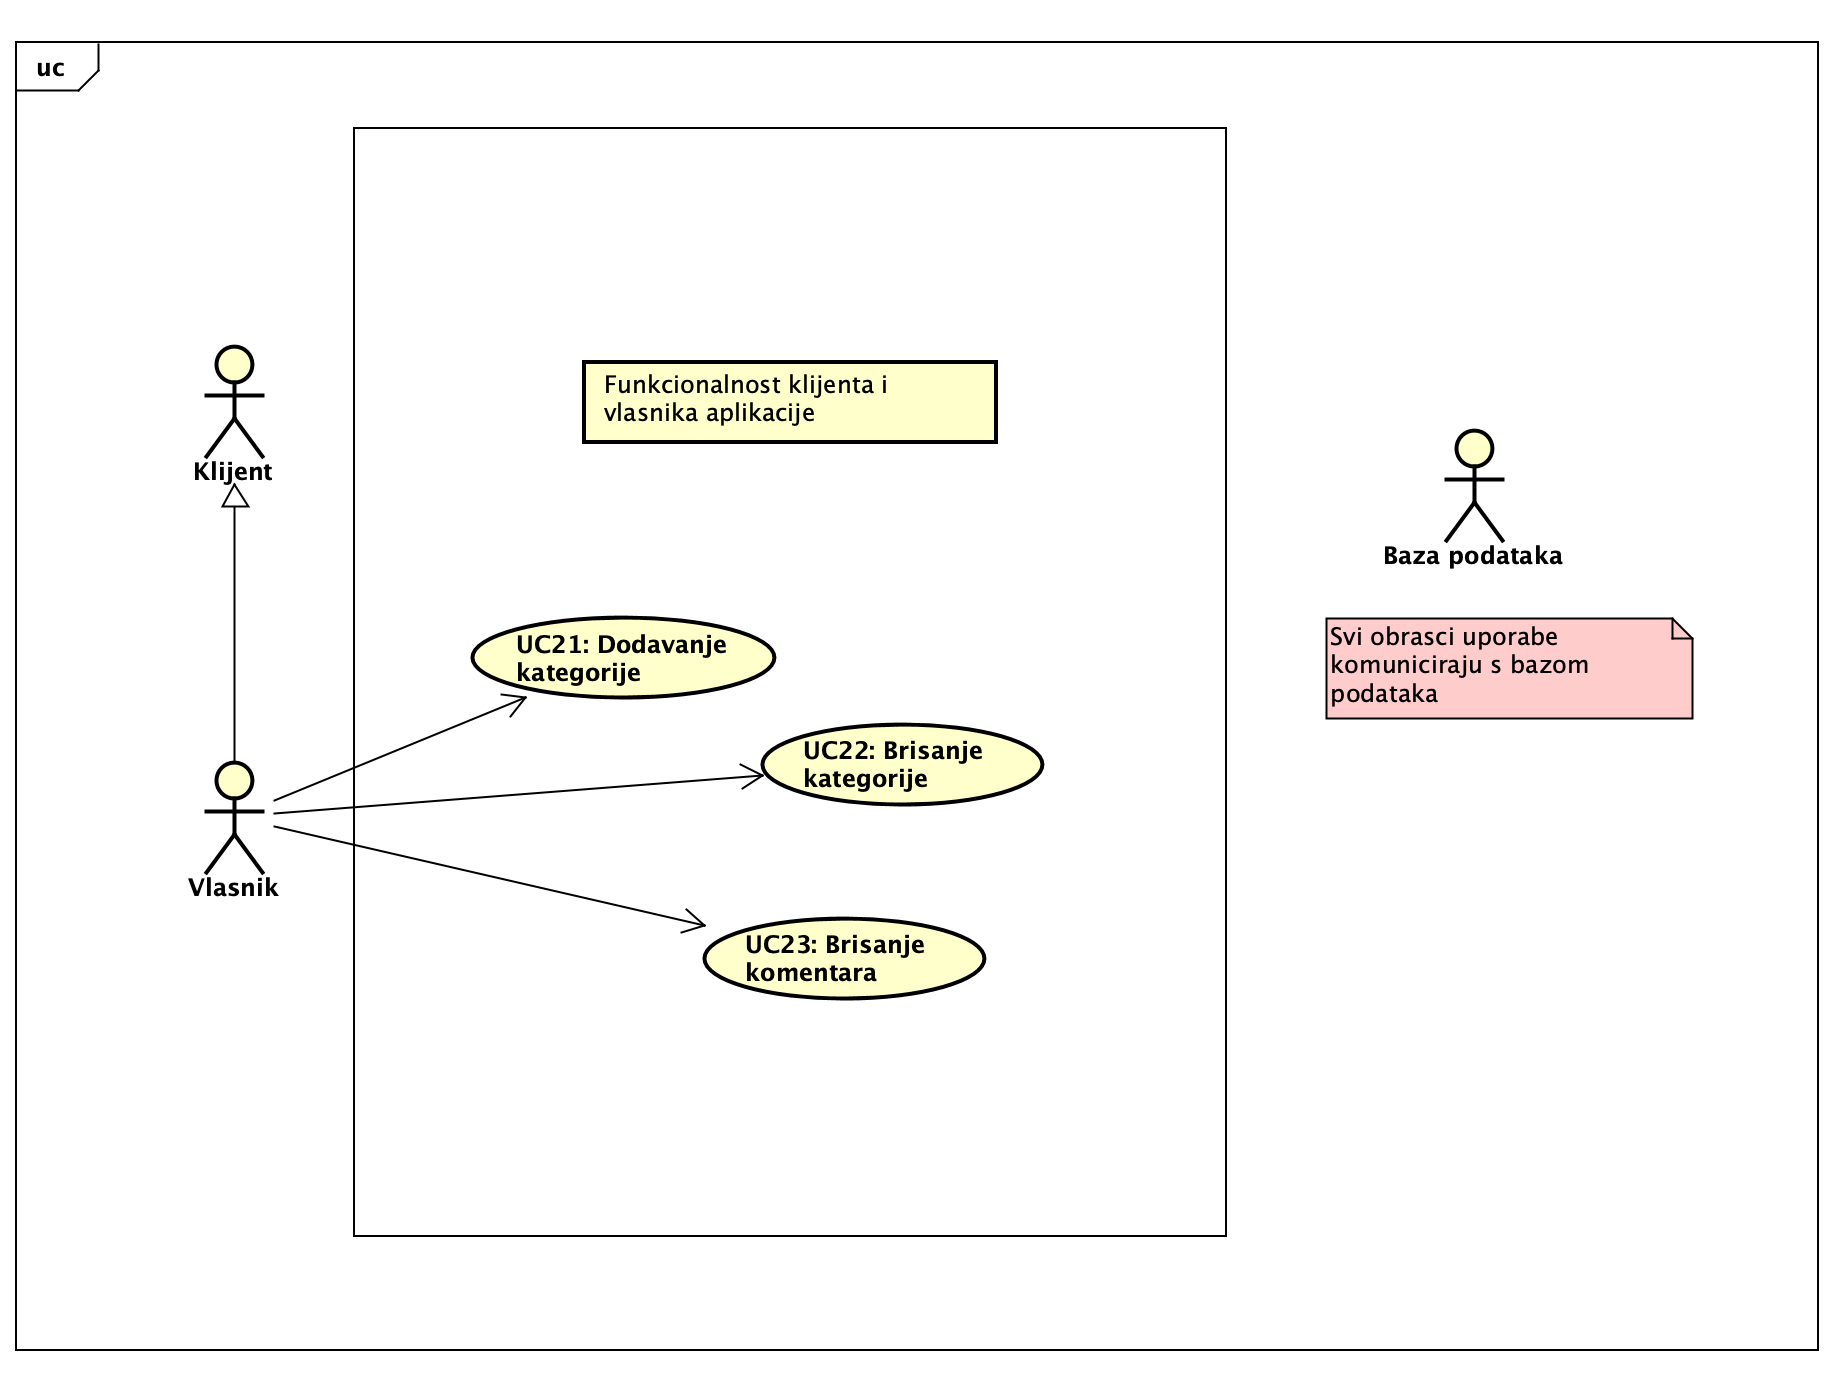
\includegraphics[scale=0.6]{dijagrami/Vlasnik.png} 
					\centering
					\caption{Dijagram obrasca uporabe, funkcionalnost vlasnika}
					\label{fig:vlasnik}
				\end{figure}		
				\eject 

				\begin{figure}[H]
					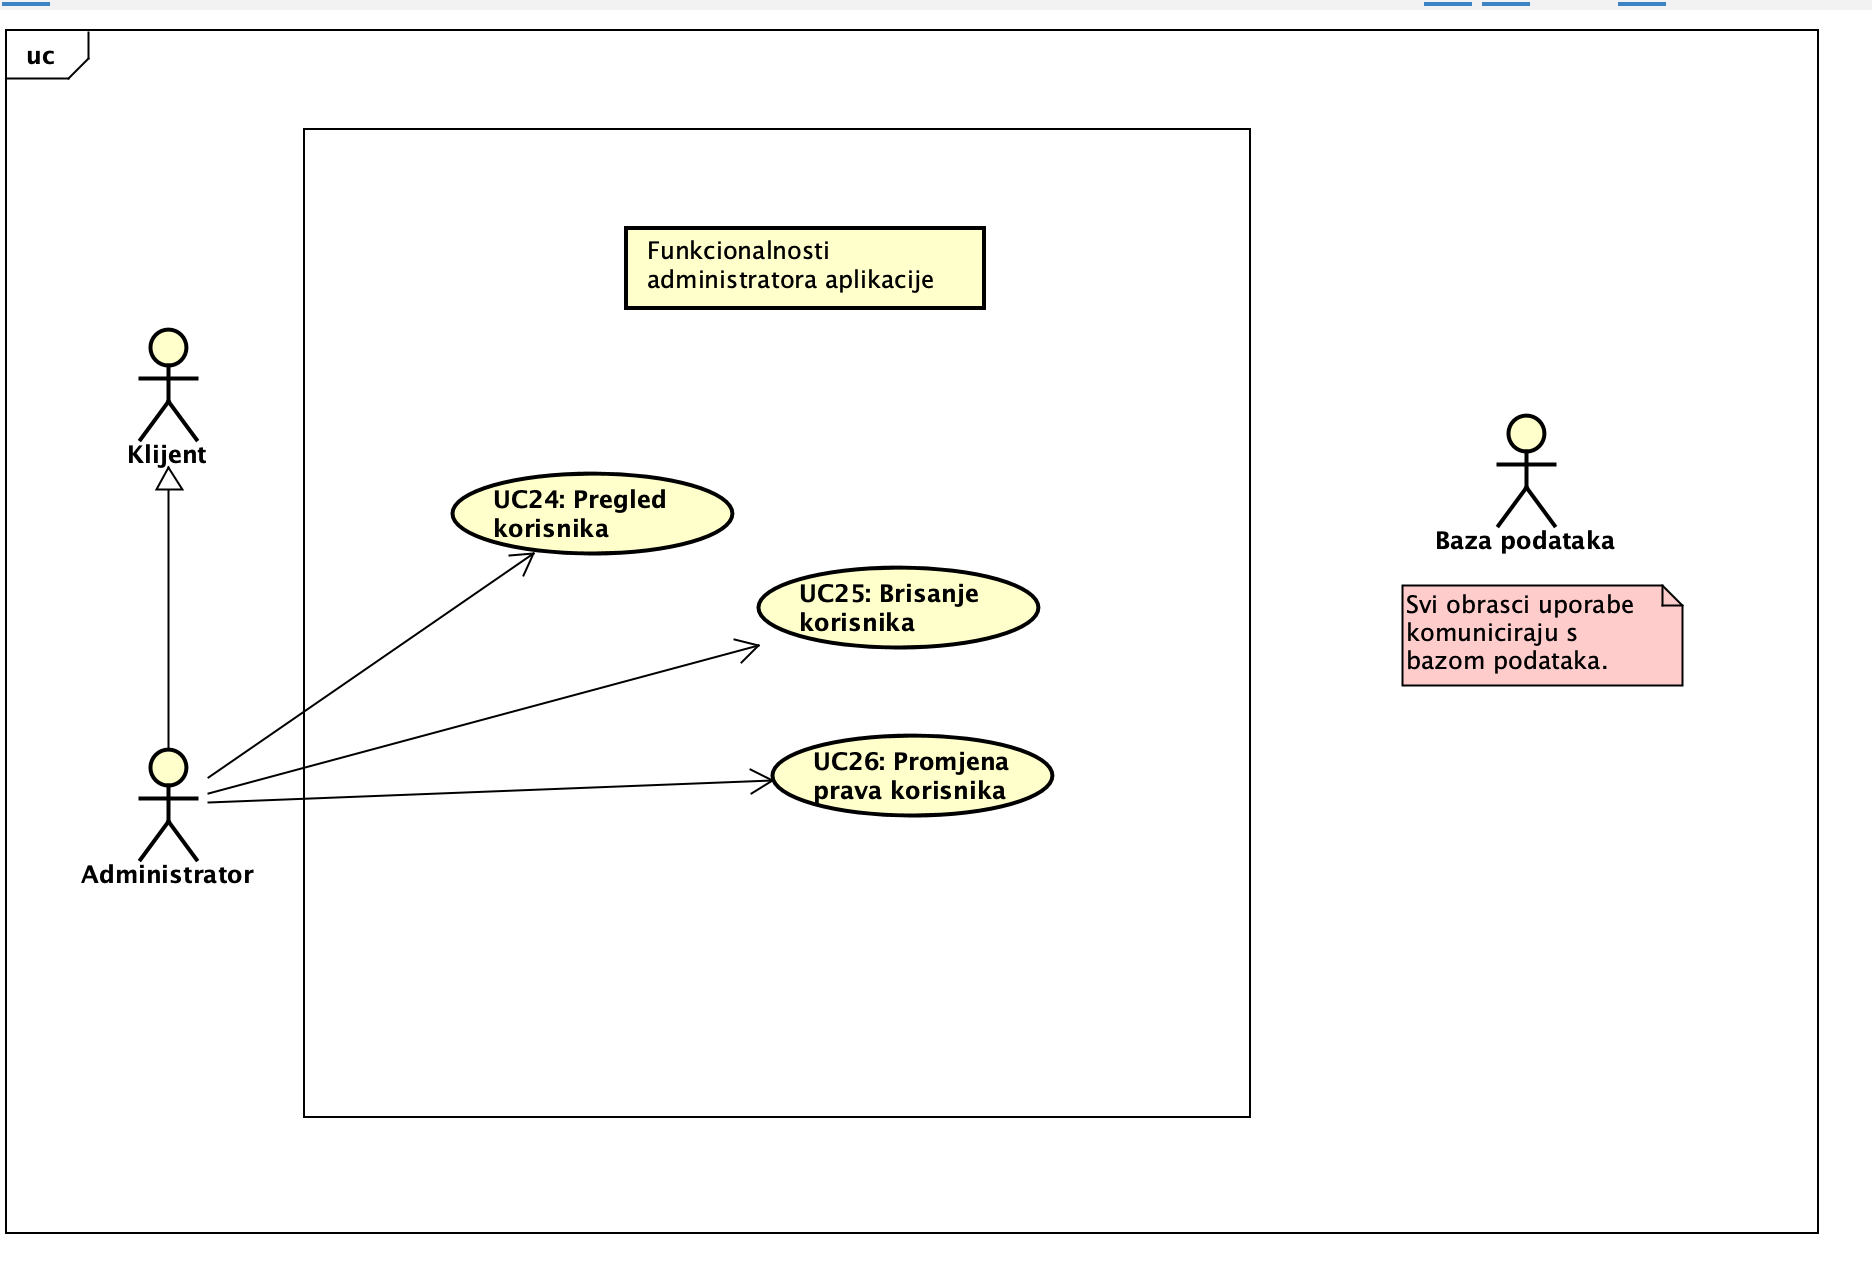
\includegraphics[scale=0.6]{dijagrami/Administrator.png} 
					\centering
					\caption{Dijagram obrasca uporabe, funkcionalnost administratora}
					\label{fig:administrator}
				\end{figure}		
				\eject 
			\subsection{Sekvencijski dijagrami}
				
				\textbf{Obrazac uporabe UC8 – Uređivanje recepta}

				Klijent šalje zahtjev za prikaz svojih recepata kako bi mogao 
				odabrati recept koji želi urediti. Poslužitelj dohvaća dostupne recepte 
				i prikazuje ih ukoliko postoje. U slučaju da ne postoji niti jedan recept 
				poslužitelj vraća odgovarajuću poruku. Odabirom recepta poslužitelj iz 
				baze podataka dohvaća podatke o receptu i prikazuje ih korisniku. 
				Korisnik unosi nove podatke o željenom receptu i šalje zahtjev za 
				promjenom. Poslužitelj izmijeni recept u bazi podataka koja vraća potvrdu.

				\begin{figure}[H]
					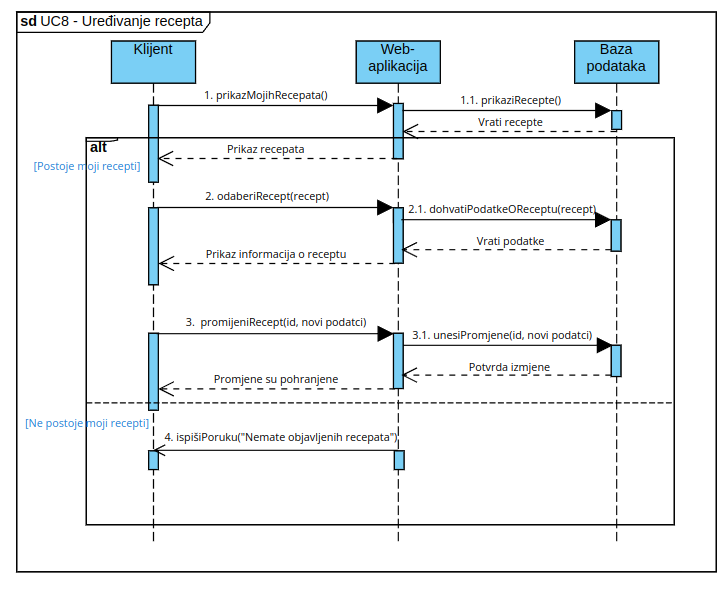
\includegraphics[scale=0.6]{dijagrami/SD8.png} 
					\centering
					\caption{Sekvencijski dijagram za UC8}
					\label{fig:sd8}
				\end{figure}		
				\eject
				
				\textbf{Obrazac uporabe UC10 – Slanje poruke}

				Klijent šalje zahtjev za prikaz recepata po kategorijama. Poslužitelj 
				dohvaća dostupne recepte i prikazuje ih ukoliko postoje. U slučaju 
				da ne postoji niti jedan recept poslužitelj vraća odgovarajuću poruku. 
				Odabirom recepta poslužitelj iz baze podataka dohvaća podatke o receptu 
				i prikazuje ih korisniku. Klijent šalje zahtjev za slanje poruke autoru 
				recepta i samu poruku. Poslužitelj prosljeđuje poruku bazi podataka koja 
				sprema poruku i vraća potvrdu što znači da je poruka poslana.
					
				\begin{figure}[H]
					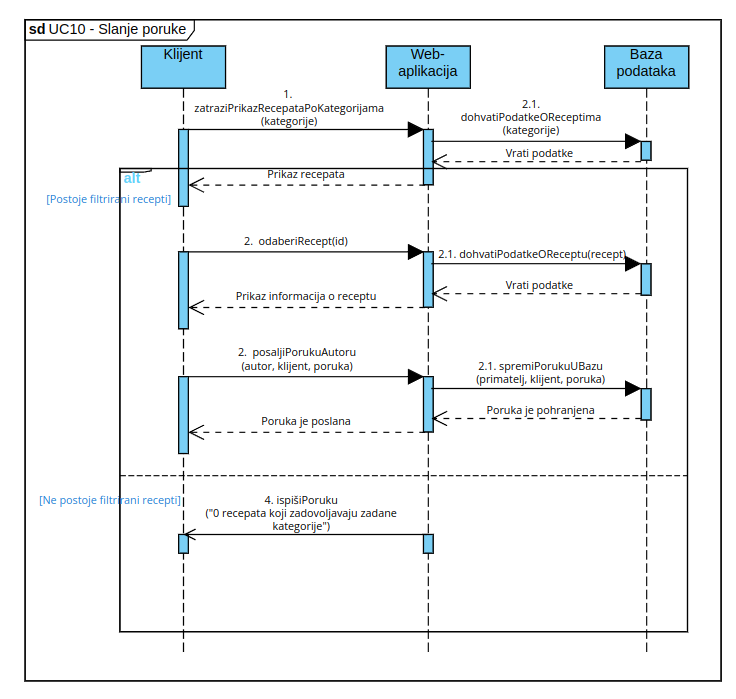
\includegraphics[scale=0.6]{dijagrami/SD10.png} 
					\centering
					\caption{Sekvencijski dijagram za UC10}
					\label{fig:sd10}
				\end{figure}		
				\eject 

				\textbf{Obrazac uporabe UC11 – Primanje poruke}

				Poslužitelj svake 2 minute u bazi podataka provjerava za prijavljenog 
				korisnika da li su pristigle neke poruke za njega. Ukoliko baza podataka 
				pošalje potvrdu da je primljena poruka poslužitelj javlja klijentu i 
				poruke se prikazuju u pretincu obavijesti.

				\begin{figure}[H]
					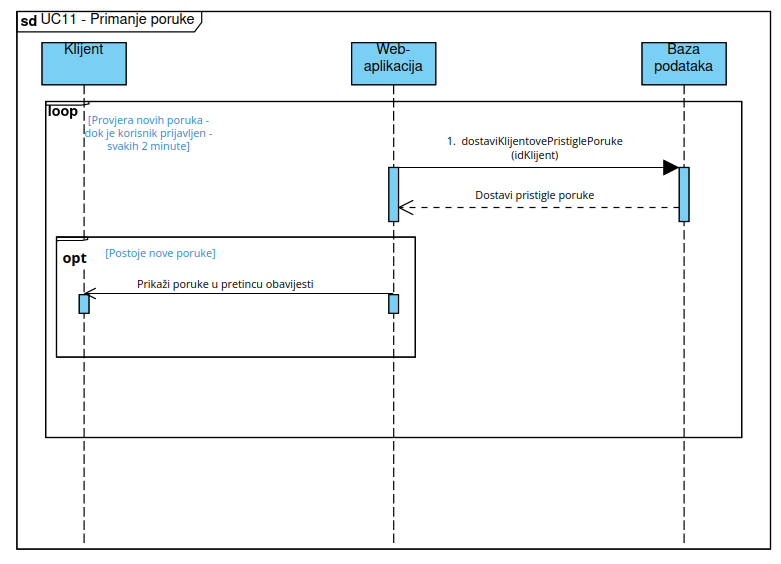
\includegraphics[scale=0.6]{dijagrami/SD11.png} 
					\centering
					\caption{Sekvencijski dijagram za UC11}
					\label{fig:sd11}
				\end{figure}		
				\eject 

				\textbf{Obrazac uporabe UC25 – Brisanje korisnika}

				Administrator traži od poslužitelja pristup popisu klijenata i ukoliko je 
				sve u redu poslužitelj vraća potvrdu i odobrava mu pristup. Zatim 
				administrator šalje zahtjev za prikaz popisa klijenata. Poslužitelj 
				prosljeđuje zahtjev bazi podataka koja šalje potvrdu i administratoru 
				se prikazuje popis klijenata. Odabirom klijenta administrator šalje zahtjev 
				za brisanjem tog klijenta iz baze podataka. Poslužitelj prosljeđuje zahtjev 
				bazi podataka koja briše odabranog klijenta i sve njegove poveznice te na 
				kraju šalje potvrdu o uspješnom brisanju.
				
				\begin{figure}[H]
					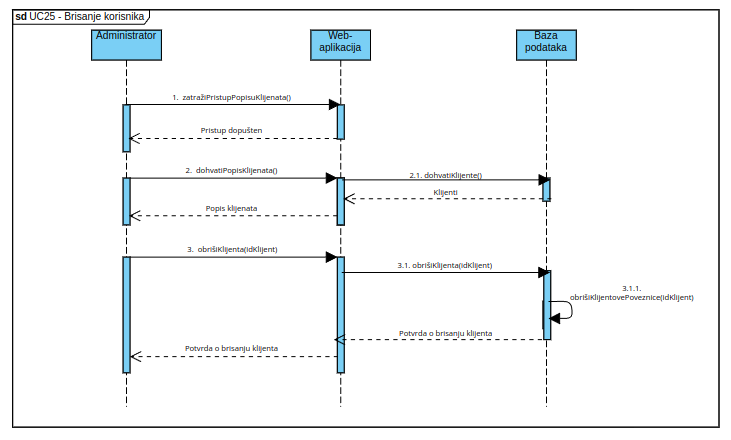
\includegraphics[scale=0.6]{dijagrami/SD25.png} 
					\centering
					\caption{Sekvencijski dijagram za UC25}
					\label{fig:sd25}
				\end{figure}		
				\eject 

	
		\section{Ostali zahtjevi}
		
			\textbf{\textit{dio 1. revizije}}\\
		 
			 \textit{Nefunkcionalni zahtjevi i zahtjevi domene primjene dopunjuju funkcionalne zahtjeve. Oni opisuju \textbf{kako se sustav treba ponašati} i koja \textbf{ograničenja} treba poštivati (performanse, korisničko iskustvo, pouzdanost, standardi kvalitete, sigurnost...). Primjeri takvih zahtjeva u Vašem projektu mogu biti: podržani jezici korisničkog sučelja, vrijeme odziva, najveći mogući podržani broj korisnika, podržane web/mobilne platforme, razina zaštite (protokoli komunikacije, kriptiranje...)... Svaki takav zahtjev potrebno je navesti u jednoj ili dvije rečenice.}
			 
			 
			 
	